\documentclass{standalone}
\usepackage{tikz}
\usetikzlibrary{patterns}
\usetikzlibrary{positioning}
\usetikzlibrary{patterns, positioning}
\usetikzlibrary{shapes.misc}
\usepackage[outline]{contour}
\contourlength{1.5pt} 
\usepackage[sfdefault]{ClearSans}

\begin{document}
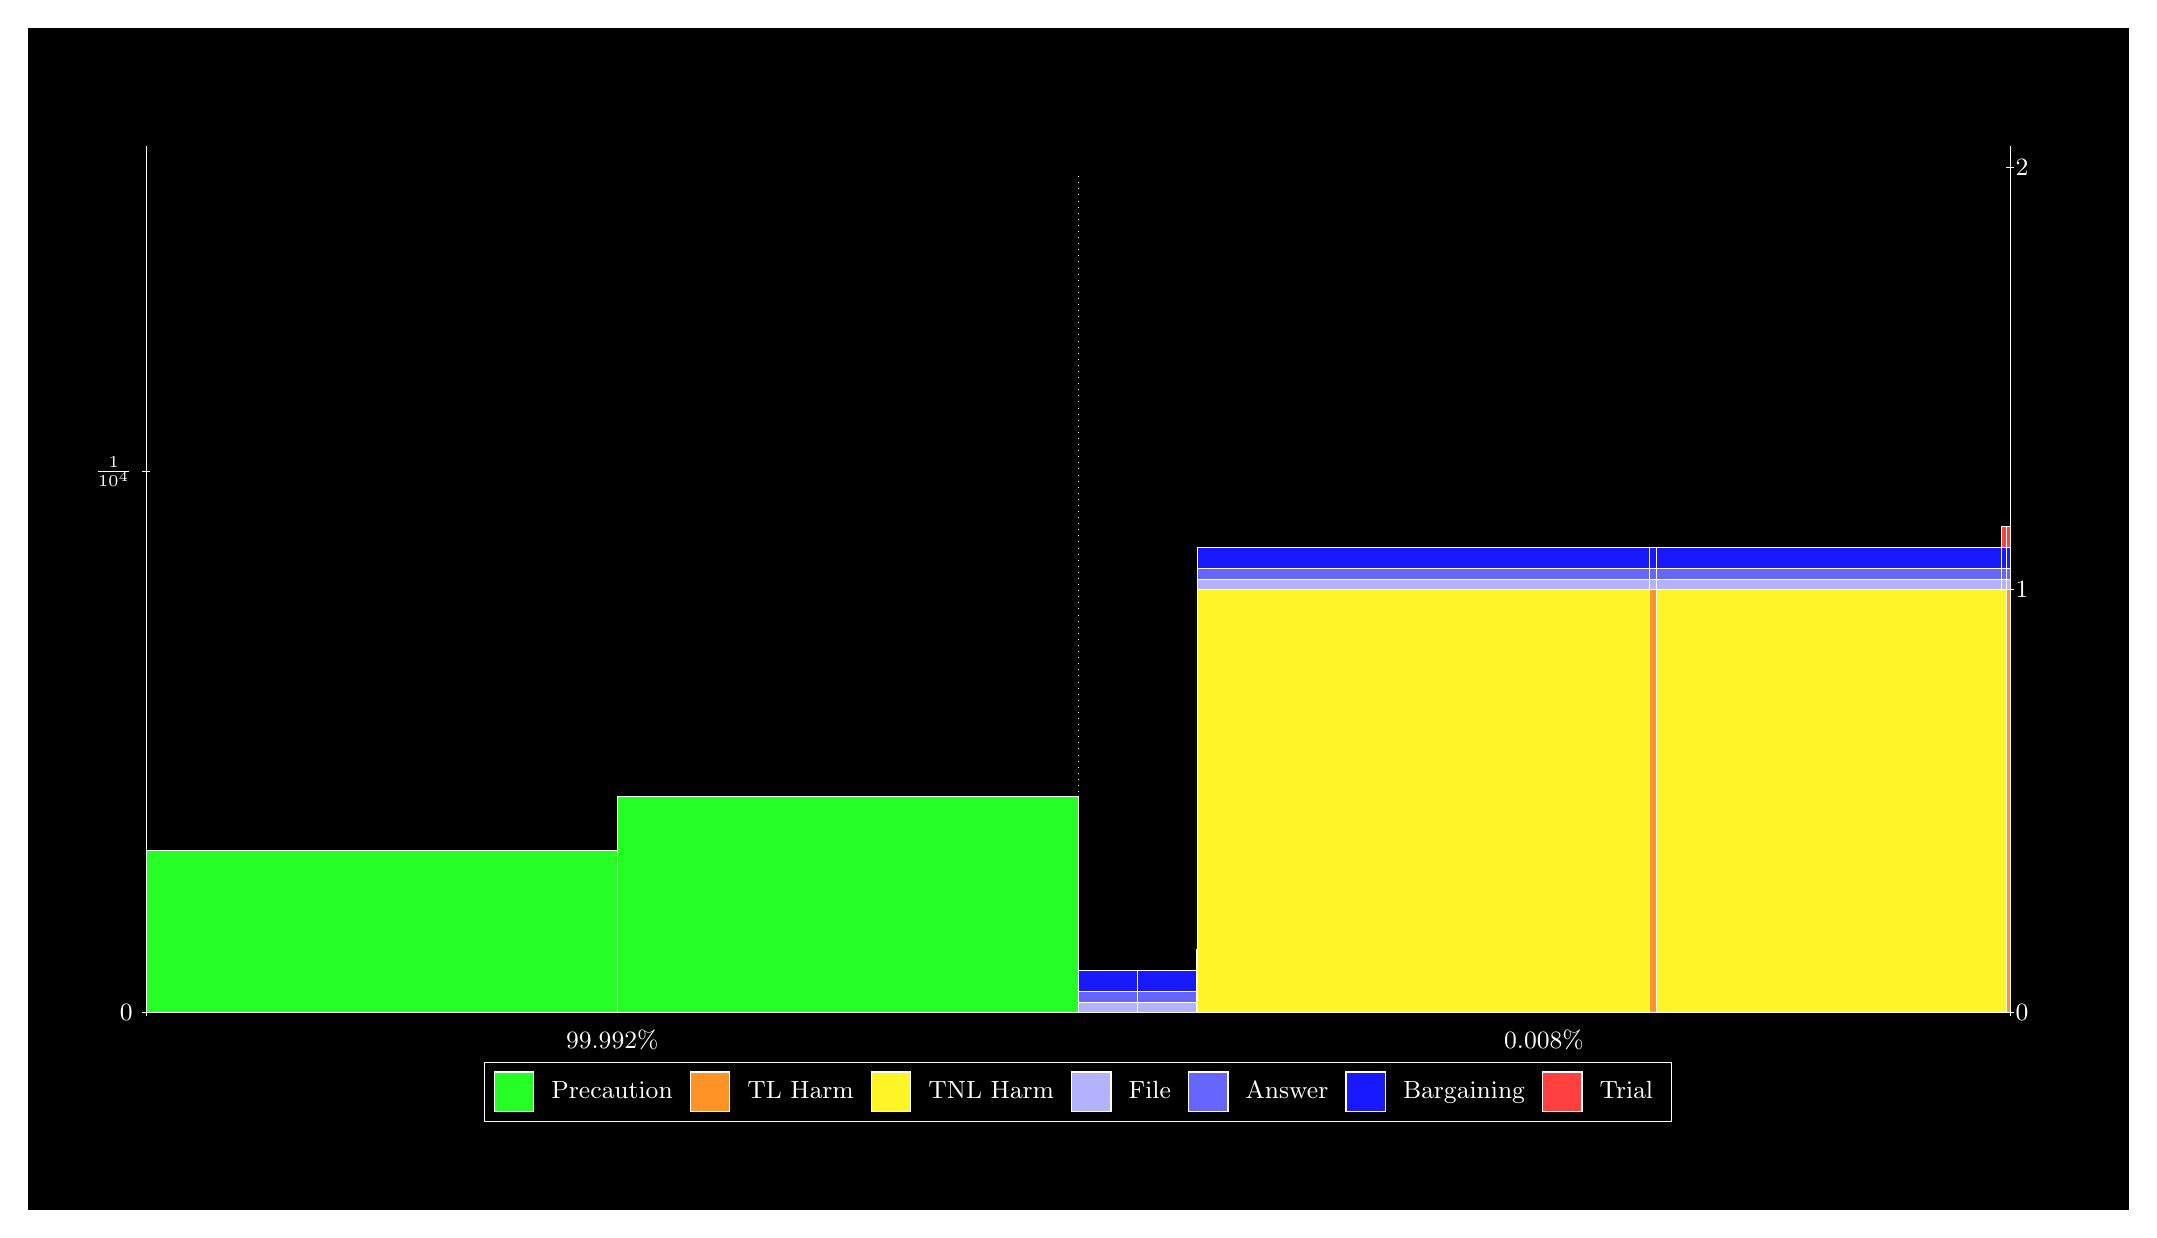
\begin{tikzpicture}
\draw[fill=black] (0,0) rectangle (26.667,15);
\draw[fill=green!85,draw=white,very thin] (1.5,2.5) rectangle (7.4844,4.5611);
\draw[fill=green!85,draw=white,very thin] (7.4844,2.5) rectangle (13.333,5.2481);
\draw[fill=green!85,draw=white,very thin] (13.333,2.5) rectangle (14.084,2.5002);
\draw[fill=blue!30,draw=white,very thin] (13.333,2.5002) rectangle (14.084,2.6344);
\draw[fill=blue!60,draw=white,very thin] (13.333,2.6344) rectangle (14.084,2.7686);
\draw[fill=blue!90,draw=white,very thin] (13.333,2.7686) rectangle (14.084,3.037);
\draw[fill=green!85,draw=white,very thin] (14.084,2.5) rectangle (14.832,2.5002);
\draw[fill=blue!30,draw=white,very thin] (14.084,2.5002) rectangle (14.832,2.6344);
\draw[fill=blue!60,draw=white,very thin] (14.084,2.6344) rectangle (14.832,2.7686);
\draw[fill=blue!90,draw=white,very thin] (14.084,2.7686) rectangle (14.832,3.0371);
\draw[fill=green!85,draw=white,very thin] (14.832,2.5) rectangle (14.848,2.5002);
\draw[fill=blue!30,draw=white,very thin] (14.832,2.5002) rectangle (14.848,2.6344);
\draw[fill=blue!60,draw=white,very thin] (14.832,2.6344) rectangle (14.848,2.7686);
\draw[fill=blue!90,draw=white,very thin] (14.832,2.7686) rectangle (14.848,3.037);
\draw[fill=red!75,draw=white,very thin] (14.832,3.037) rectangle (14.848,3.3054);
\draw[fill=green!85,draw=white,very thin] (14.848,2.5) rectangle (20.582,2.5002);
\draw[fill=yellow!85,draw=white,very thin] (14.848,2.5002) rectangle (20.582,7.8687);
\draw[fill=blue!30,draw=white,very thin] (14.848,7.8687) rectangle (20.582,8.0029);
\draw[fill=blue!60,draw=white,very thin] (14.848,8.0029) rectangle (20.582,8.1371);
\draw[fill=blue!90,draw=white,very thin] (14.848,8.1371) rectangle (20.582,8.4055);
\draw[fill=green!85,draw=white,very thin] (20.582,2.5) rectangle (20.679,2.5002);
\draw[fill=orange!85,draw=white,very thin] (20.582,2.5002) rectangle (20.679,7.8687);
\draw[fill=blue!30,draw=white,very thin] (20.582,7.8687) rectangle (20.679,8.0029);
\draw[fill=blue!60,draw=white,very thin] (20.582,8.0029) rectangle (20.679,8.1371);
\draw[fill=blue!90,draw=white,very thin] (20.582,8.1371) rectangle (20.679,8.4055);
\draw[fill=green!85,draw=white,very thin] (20.679,2.5) rectangle (25.063,2.5002);
\draw[fill=yellow!85,draw=white,very thin] (20.679,2.5002) rectangle (25.063,7.8687);
\draw[fill=blue!30,draw=white,very thin] (20.679,7.8687) rectangle (25.063,8.003);
\draw[fill=blue!60,draw=white,very thin] (20.679,8.003) rectangle (25.063,8.1372);
\draw[fill=blue!90,draw=white,very thin] (20.679,8.1372) rectangle (25.063,8.4056);
\draw[fill=green!85,draw=white,very thin] (25.063,2.5) rectangle (25.126,2.5002);
\draw[fill=yellow!85,draw=white,very thin] (25.063,2.5002) rectangle (25.126,7.8687);
\draw[fill=blue!30,draw=white,very thin] (25.063,7.8687) rectangle (25.126,8.0029);
\draw[fill=blue!60,draw=white,very thin] (25.063,8.0029) rectangle (25.126,8.1371);
\draw[fill=blue!90,draw=white,very thin] (25.063,8.1371) rectangle (25.126,8.4055);
\draw[fill=red!75,draw=white,very thin] (25.063,8.4055) rectangle (25.126,8.674);
\draw[fill=green!85,draw=white,very thin] (25.126,2.5) rectangle (25.167,2.5002);
\draw[fill=orange!85,draw=white,very thin] (25.126,2.5002) rectangle (25.167,7.8687);
\draw[fill=blue!30,draw=white,very thin] (25.126,7.8687) rectangle (25.167,8.0029);
\draw[fill=blue!60,draw=white,very thin] (25.126,8.0029) rectangle (25.167,8.1371);
\draw[fill=blue!90,draw=white,very thin] (25.126,8.1371) rectangle (25.167,8.4055);
\draw[fill=red!75,draw=white,very thin] (25.126,8.4055) rectangle (25.167,8.674);
\draw[white,very thin] (1.5,2.5) -- (1.5,13.5);
\draw[white,very thin] (1.45,2.5) -- (1.55,2.5);
\node[font=\small,text=white, anchor=east] at (1.45, 2.5) {0};
\draw[white,very thin] (1.45,9.3702) -- (1.55,9.3702);
\node[font=\small,text=white, anchor=east] at (1.45, 9.3702) {$\frac{1}{10^{4}}$};

\draw[white,dotted,very thin] (13.333,2.83) -- (13.333,13.17);
\draw[white,very thin] (25.167,2.5) -- (25.167,13.5);
\draw[white,very thin] (25.117,2.5) -- (25.217,2.5);
\node[font=\small,text=white, anchor=west] at (25.117, 2.5) {0};
\draw[white,very thin] (25.117,7.8685) -- (25.217,7.8685);
\node[font=\small,text=white, anchor=west] at (25.117, 7.8685) {1};
\draw[white,very thin] (25.117,13.237) -- (25.217,13.237);
\node[font=\small,text=white, anchor=west] at (25.117, 13.237) {2};

\draw[white,very thin] (1.5,2.5) -- (25.167,2.5);
\draw[white,very thin] (1.5,2.45) -- (1.5,2.55);
\node[font=\small,text=white, anchor=north] at (1.5, 2.45) {};
\draw[white,very thin] (25.167,2.45) -- (25.167,2.55);
\node[font=\small,text=white, anchor=north] at (25.167, 2.45) {};

\node[font=\small,text=white,anchor=south] at (7.4167, 1.9) {99.992\%};
\node[font=\small,text=white,anchor=south] at (19.25, 1.9) {0.008\%};
\draw (13.3333,2.5) node (B) {};
\begin{scope}[align=center]
\matrix[scale=0.5,draw=white,below=0.5cm of B,nodes={draw},column sep=0.1cm]{
\node[rectangle,draw,minimum width=0.5cm,minimum height=0.5cm,fill=green!85]{}; & \node[draw=none,font=\small,text=white]{Precaution}; &
\node[rectangle,draw,minimum width=0.5cm,minimum height=0.5cm,fill=orange!85]{}; & \node[draw=none,font=\small,text=white]{TL Harm}; &
\node[rectangle,draw,minimum width=0.5cm,minimum height=0.5cm,fill=yellow!85]{}; & \node[draw=none,font=\small,text=white]{TNL Harm}; &
\node[rectangle,draw,minimum width=0.5cm,minimum height=0.5cm,fill=blue!30]{}; & \node[draw=none,font=\small,text=white]{File}; &
\node[rectangle,draw,minimum width=0.5cm,minimum height=0.5cm,fill=blue!60]{}; & \node[draw=none,font=\small,text=white]{Answer}; &
\node[rectangle,draw,minimum width=0.5cm,minimum height=0.5cm,fill=blue!90]{}; & \node[draw=none,font=\small,text=white]{Bargaining}; &
\node[rectangle,draw,minimum width=0.5cm,minimum height=0.5cm,fill=red!75]{}; & \node[draw=none,font=\small,text=white]{Trial}; \\\\
};\end{scope}

\end{tikzpicture}
\end{document}